\documentclass[border=10pt]{standalone}
\usepackage[svgnames]{xcolor}
\usepackage{amsmath}
\usepackage{pgfplots}
\pgfplotsset{compat=newest}
\usepackage[sfdefault]{FiraSans}
\usepackage{FiraMono}
\renewcommand*\familydefault{\sfdefault}
\begin{document}
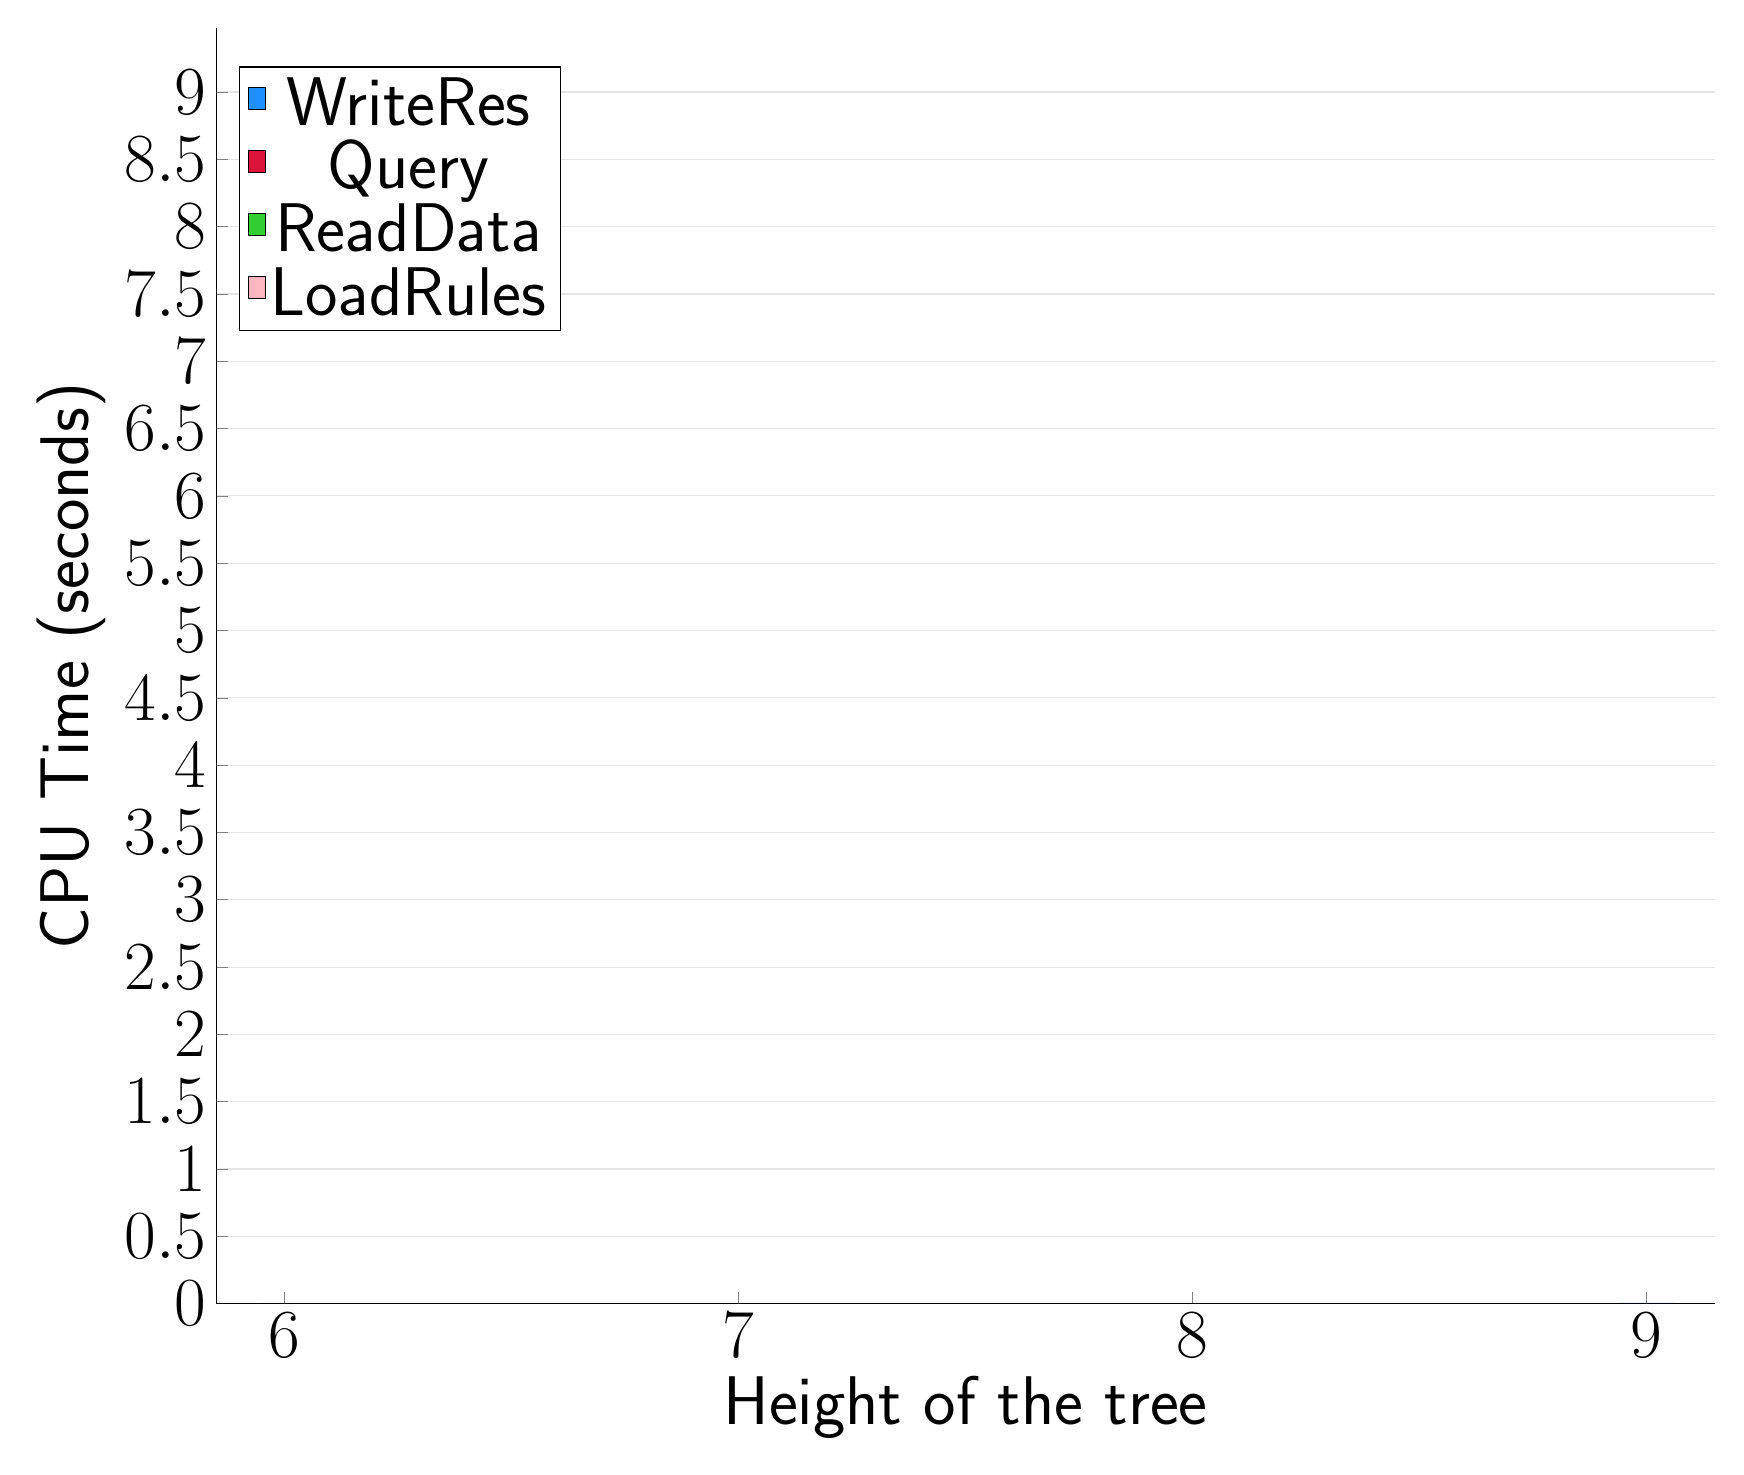
\begin{tikzpicture}
\begin{axis}[
   ybar stacked,
   width=1.7\textwidth,
   bar width=0.7cm,
   ymajorgrids, tick align=inside,
   major grid style={draw=gray!20},
   xtick=data,
   ymin=0, ymax=9.474,
   axis x line*=bottom,
   axis y line*=left,
   enlarge x limits=0.05,
   legend style={
       at={(0.23, 0.97)},
       anchor=north east,
       legend columns=1,
       font=\Huge,
   },
   ylabel={CPU Time (seconds)},
   xlabel={Height of the tree},
   label style={font=\Huge},
   tick label style={font=\Huge},
]
\addlegendimage{fill=DodgerBlue, draw=black, line width=0.2pt}
\addlegendentry{WriteRes}
\addlegendimage{fill=Crimson, draw=black, line width=0.2pt}
\addlegendentry{Query}
\addlegendimage{fill=LimeGreen, draw=black, line width=0.2pt}
\addlegendentry{ReadData}
\addlegendimage{fill=LightPink, draw=black, line width=0.2pt}
\addlegendentry{LoadRules}
\addplot +[fill=LightPink, draw=black, line width=0.2pt] coordinates {
(6, 0.0005516000000000002)
(7, 0.0005479999999999997)
(8, 0.0005490000000000004)
(8, 0.0005482000000000002)
(8, 0.0005512000000000002)
(9, 0.0005494000000000001)
(9, 0.0005516000000000002)
(9, 0.0005478000000000004)
(9, 0.0005499999999999998)
(9, 0.0005481999999999998)
};
\addplot +[fill=LimeGreen, draw=black, line width=0.2pt] coordinates {
(6, 0.00017019999999999983)
(7, 0.0002182000000000002)
(8, 0.0003174)
(8, 0.0003201999999999998)
(8, 0.0003201999999999996)
(9, 0.0005212000000000001)
(9, 0.0005228000000000006)
(9, 0.0005189999999999997)
(9, 0.0005202)
(9, 0.0005170000000000006)
};
\addplot +[fill=Crimson, draw=black, line width=0.2pt] coordinates {
(6, 5.8199999999999605e-05)
(7, 0.00013359999999999983)
(8, 0.000332)
(8, 0.0003336000000000004)
(8, 0.0003347999999999994)
(9, 0.0008299999999999998)
(9, 0.0008289999999999992)
(9, 0.0008361999999999999)
(9, 0.0008271999999999998)
(9, 0.0008342)
};
\addplot +[fill=DodgerBlue, draw=black, line width=0.2pt] coordinates {
(6, 0.0002762000000000006)
(7, 0.0006027999999999995)
(8, 0.0013637999999999999)
(8, 0.0013721999999999994)
(8, 0.0013612000000000006)
(9, 0.0030948000000000004)
(9, 0.0031034000000000005)
(9, 0.0030666)
(9, 0.0031056000000000005)
(9, 0.0030934)
};
\end{axis}
\end{tikzpicture}

\end{document}
